
\documentclass[11pt]{article}
\usepackage[T1]{fontenc}
\usepackage{amsmath,amssymb}
\usepackage[margin=1in]{geometry}
\usepackage[table]{xcolor}
\usepackage{graphicx}
\usepackage{array}
\usepackage{booktabs}
\usepackage{float}
\usepackage{caption}
\usepackage{tikz}
\title{Tables, Color, and Figures in LaTeX}
\author{}
\date{}
\begin{document}
\maketitle
\tableofcontents
\bigskip

\section{Creating a Basic Table}
\textbf{Definition.} The \texttt{tabular} environment creates a table. The column format tells LaTeX how many columns there are and how to align them. The letter \texttt{l} means left, \texttt{c} means centered, and \texttt{r} means right.

\textbf{Source code:}
\begin{verbatim}
\begin{tabular}{|l|c|r|}
\hline
Name & Subject & Marks \\
\hline
Asha & Maths & 95 \\
Ravi & Science & 88 \\
\hline
\end{tabular}
\end{verbatim}

\textbf{Expected result:}
\[
\begin{array}{|l|c|r|}
\hline
\text{Name} & \text{Subject} & \text{Marks}\\
\hline
\text{Asha} & \text{Maths} & 95\\
\text{Ravi} & \text{Science} & 88\\
\hline
\end{array}
\]

\textbf{Commands.} Use \texttt{\&} to separate columns, \texttt{\textbackslash\textbackslash} to start a new row, and \texttt{\textbackslash hline} to draw a horizontal line.

\textbf{Practice.} Create a table with three columns: item, quantity, and price.

\section{Improving Tables with Booktabs}
\textbf{Definition.} The \texttt{booktabs} package provides cleaner horizontal rules for professional-looking tables. Its main commands are \texttt{\textbackslash toprule}, \texttt{\textbackslash midrule}, and \texttt{\textbackslash bottomrule}.

\textbf{Source code:}
\begin{verbatim}
\begin{tabular}{lcr}
\toprule
Name & Level & Score \\
\midrule
Mina & Beginner & 82 \\
Omar & Advanced & 96 \\
\bottomrule
\end{tabular}
\end{verbatim}

\textbf{Expected result:}
\begin{center}
\begin{tabular}{lcr}
\toprule
Name & Level & Score \\
\midrule
Mina & Beginner & 82 \\
Omar & Advanced & 96 \\
\bottomrule
\end{tabular}
\end{center}

\textbf{Commands.} Add \texttt{\textbackslash usepackage\{booktabs\}} in the preamble. Prefer these rules instead of drawing a box around every cell.

\textbf{Practice.} Make a booktabs table comparing three programming languages.

\section{Adding Color to Text}
\textbf{Definition.} The \texttt{xcolor} package allows text and other elements to be colored. The command \texttt{\textbackslash textcolor} applies a color to a selected piece of text.

\textbf{Source code:}
\begin{verbatim}
\textcolor{red}{This text is red.}

\textcolor{blue}{This text is blue.}

\textcolor{teal}{This text is teal.}
\end{verbatim}

\textbf{Expected result:}

\textcolor{red}{This text is red.}

\textcolor{blue}{This text is blue.}

\textcolor{teal}{This text is teal.}

\textbf{Commands.} Load the package with \texttt{\textbackslash usepackage\{xcolor\}}. The syntax is \texttt{\textbackslash textcolor\{color\}\{text\}}. Many standard color names are available.

\textbf{Practice.} Write one sentence in green and another in purple.

\section{Highlighting Table Rows and Cells}
\textbf{Definition.} With \texttt{xcolor}'s table support, you can shade an individual cell or an entire row. This can make headings and important values easier to notice.

\textbf{Source code:}
\begin{verbatim}
\begin{tabular}{|l|c|}
\hline
\rowcolor{lightgray}
Product & Stock \\
\hline
Notebook & 24 \\
\cellcolor{yellow}Pen & 50 \\
\hline
\end{tabular}
\end{verbatim}

\textbf{Expected result:}
\begin{center}
\begin{tabular}{|l|c|}
\hline
\rowcolor{lightgray}
Product & Stock \\
\hline
Notebook & 24 \\
\cellcolor{yellow}Pen & 50 \\
\hline
\end{tabular}
\end{center}

\textbf{Commands.} Use \texttt{\textbackslash rowcolor\{lightgray\}} immediately after the row begins to shade a row. Use \texttt{\textbackslash cellcolor\{yellow\}} inside a cell to shade only that cell.

\textbf{Practice.} Shade the heading row of your own table and highlight one important cell.

\section{Including an Image}
\textbf{Definition.} The \texttt{graphicx} package provides the \texttt{\textbackslash includegraphics} command for inserting image files. Keep the image file in the same folder as your \texttt{.tex} file, or provide its relative path.

\textbf{Source code:}
\begin{verbatim}
\usepackage{graphicx}

\begin{figure}
\centering
\includegraphics[width=0.6\textwidth]{example-image}
\caption{An example image}
\label{fig:example}
\end{figure}
\end{verbatim}

\textbf{Expected result:} A centered image appears at 60\% of the text width, with the caption ``An example image'' below it. The sample filename \texttt{example-image} is supplied by many LaTeX installations; replace it with your own image filename, such as \texttt{photo.png}.

\textbf{Commands.} The \texttt{width} option controls image size. The \texttt{figure} environment creates a floating figure. Use \texttt{\textbackslash centering} to center it, \texttt{\textbackslash caption} to add a caption, and \texttt{\textbackslash label} to give it a reference name.

\textbf{Practice.} Insert an image named \texttt{myphoto.png} and give it a meaningful caption.

\section{Figure Placement and Resizing}
\textbf{Definition.} Figures are floats, so LaTeX may move them to improve page layout. Placement options suggest where a figure should appear: \texttt{h} means here, \texttt{t} top, \texttt{b} bottom, and \texttt{p} a page of floats. The exclamation mark asks LaTeX to be less restrictive.

\textbf{Source code:}
\begin{verbatim}
\begin{figure}[htbp]
\centering
\includegraphics[width=0.45\textwidth]{example-image}
\caption{A resized figure}
\label{fig:resized}
\end{figure}
\end{verbatim}

\textbf{Expected result:} The image is displayed at 45\% of the text width, with a caption. LaTeX chooses a suitable location, preferring here, top, bottom, or a float page.

\textbf{Commands.} Change the width to \texttt{0.8\textbackslash textwidth} for a larger image. Avoid forcing every figure into an exact position unless there is a good reason.

\textbf{Practice.} Add a second figure and set its width to 30\% of the text width.

\section{Referencing Figures and Tables}
\textbf{Definition.} A label lets you refer to a numbered figure or table elsewhere in the document. Use \texttt{\textbackslash ref} to print its number. LaTeX may need to be compiled twice to update references.

\textbf{Source code:}
\begin{verbatim}
Figure~\ref{fig:example} shows the sample image.

\begin{figure}
\centering
\includegraphics[width=0.4\textwidth]{example-image}
\caption{Sample image for reference}
\label{fig:example}
\end{figure}
\end{verbatim}

\textbf{Expected result:} The sentence refers to the figure number automatically, for example, ``Figure 1 shows the sample image.''

\textbf{Commands.} Put \texttt{\textbackslash label} after \texttt{\textbackslash caption} so the label records the correct figure number. The same approach works for tables.

\textbf{Practice.} Add a table caption and label, then refer to it in a sentence using \texttt{\textbackslash ref}.

\section{A Complete Mini Example}
The following example combines a colored heading, a table, and a figure. The TikZ drawing is used here so the example compiles without needing an external image file.

\textbf{Source code:}
\begin{verbatim}
\textcolor{blue}{\Large My Project Summary}

\begin{tabular}{lr}
\toprule
Task & Hours \\
\midrule
Planning & 3 \\
Writing & 5 \\
Review & 2 \\
\bottomrule
\end{tabular}

\begin{figure}[H]
\centering
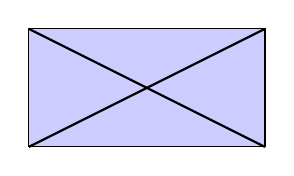
\begin{tikzpicture}
\draw[fill=blue!20] (0,0) rectangle (3,1.5);
\draw[thick] (0,0) -- (3,1.5);
\draw[thick] (0,1.5) -- (3,0);
\end{tikzpicture}
\caption{A simple project illustration}
\end{figure}
\end{verbatim}

\textbf{Expected result:}

\textcolor{blue}{\Large My Project Summary}

\begin{center}
\begin{tabular}{lr}
\toprule
Task & Hours \\
\midrule
Planning & 3 \\
Writing & 5 \\
Review & 2 \\
\bottomrule
\end{tabular}
\end{center}

\begin{center}
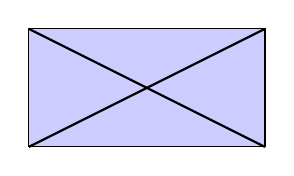
\begin{tikzpicture}
\draw[fill=blue!20] (0,0) rectangle (3,1.5);
\draw[thick] (0,0) -- (3,1.5);
\draw[thick] (0,1.5) -- (3,0);
\end{tikzpicture}

\textbf{Figure:} A simple project illustration
\end{center}

\textbf{Practice.} Create a one-page report containing a colored title, a table with at least three rows, and one labeled figure.

\end{document}
